%%==================================================
%% diss.tex for SJTU Master Thesis
%% based on CASthesis
%% modified by wei.jianwen@gmail.com
%% version: 0.3a
%% Encoding: UTF-8
%% last update: Dec 5th, 2010
%%==================================================

% 字号选项: c5size 五号(默认)
% 字号选项: cs4size 小四
% 双面打印(注意字号设置)
\documentclass[cs4size, a4paper, cs4size, twoside]{sjtumaster-xetex} 
% 单面打印(注意字号设置)
% \documentclass[cs4size, a4paer, cs4size, oneside, openany]{sjtumaster-xetex} 


% \usepackage[sectionbib]{chapterbib}%每章都用参考文献

\newboolean{DOIT}
\setboolean{DOIT}{false}%编译某些只想自己看的内容,编译true,否则false

%% 行距缩放因子(x倍字号)
\renewcommand{\baselinestretch}{1.3}

% 设置图形文件的搜索路径
\graphicspath{{figure/}{figures/}{logo/}{logos/}{graph/}{graphs}}

%%========================================
%% 在sjtumaster-xetex.cls中定义的有用命令
%%========================================
% \cndash 中文破折号
% 数学常量
% \me 对数常数e
% \mi 虚数单位i
% \mj 虚数单位j
% \dif 直立的微分算符d为直立体。
% 可伸长的数学箭头、等号
% \myRightarrow{}{}
% \myLeftarrow{}{}
% \myBioarrow{}{}
% \myLongEqual{}{}
% 参考文献
% \upcite{} 上标引用
%%========================================


\begin{document}

%%%%%%%%%%%%%%%%%%%%%%%%%%%%%% 
%% 封面
%%%%%%%%%%%%%%%%%%%%%%%%%%%%%% 

% 中文封面内容(关注内容而不是形式)
\title{上海交通大学硕士学位论文~\XeTeX/\LaTeX~模板~\version}
\author{李\quad{}四}
\advisor{张三教授}
\degree{硕士}
\defenddate{2010年1月16日}
\school{上海交通大学}
\institute{物理系}
\studentnumber{0010900990}
\major{专业名称}

% 英文封面内容(关注内容而不是表现形式)
\englishtitle{\XeTeX/\LaTeX\, Template for SJTU Mater Degree Thesis \version}
\englishauthor{\textsc{Si Li}}
\englishadvisor{Prof. \textsc{San Zhang}}
\englishschool{Shanghai Jiao Tong University}
\englishinstitute{\textsc{Depart of XXX, School of XXX} \\
  \textsc{Shanghai Jiao Tong University} \\
  \textsc{Shanghai, P.R.China}}
\englishdegree{Master}
\englishmajor{Physics}
\englishdate{Jan. 16th, 2010}

% 封面
\maketitle

% 英文封面
\makeenglishtitle

% 论文原创性声明和使用授权
\makeDeclareOriginal
\makeDeclareAuthorization

%%%%%%%%%%%%%%%%%%%%%%%%%%%%%% 
%% 前言
%%%%%%%%%%%%%%%%%%%%%%%%%%%%%% 
\frontmatter

% 摘要
%%==================================================
%% abstract.tex for SJTU Master Thesis
%% based on CASthesis
%% modified by wei.jianwen@gmail.com
%% version: 0.3a
%% Encoding: UTF-8
%% last update: Dec 5th, 2010
%%==================================================

\begin{abstract}

  上海交通大学是我国历史最悠久的高等学府之一,是教育部直属、教育部与上海市共建的全国重点大学,是国家 “七五”、“八五”重点建设和“211工程”、“985工程”的首批建设高校。经过113年的不懈努力,上海交通大学已经成为一所“综合性、研究型、国际化”的国内一流、国际知名大学,并正在向世界一流大学稳步迈进。
  学校现有本科专业67个,涵盖经济学、法学、文学、理学、工学、农学、医学和管理学等8个学科门类;拥有工科物理、工科数学和电工电子等3个国家工科基础课程教学基地,生命科学和集成电路等2个国家人才培养基地和教育部大学生文化素质教育基地,以及国家生物学理科人才培养基地;有国家级实验教学示范中心5个,上海市实验教学示范中心4个;有国家级教学团队5个,上海市级教学团队9各;有国家级教学名师奖获得者6人,上海市教学名师奖获得者32人;有国家级精品课程40门,上海市精品课程100门;有国家级双语示范课程5门;2005年和2009年,作为第一完成单位,共获得国家级教学成果22项、上海市级教学成果105项。

  \keywords{\large 上海交大 \quad 饮水思源 \quad 爱国荣校}
\end{abstract}

\begin{englishabstract}

  Shanghai Jiao Tong University (SJTU), directly subordinate to the Ministry of Education, is a key university in China, jointly run by the Ministry and Shanghai Municipality.
  SJTU has beautiful campuses, occupying an area of more than 200 hectare in total, and possesses plenty of advanced teaching and research equipment and facilities. Now, it has six campuses, the Xuhui, the Minhang, the Qibao, the Shangzhong Road , the Fahuazheng Road and the Chongqing Road(south). Over the past decade, the number of students in SJTU has grown from 5,000 to more than 38,000, the floorage of various buildings from 230,000 square meters to 800,000 square meters, and the area of campuses from 40ha to 200ha. Apart from the major buildings such as the Lecture Buildings, Laboratory Buildings, Dormitories and Gymnasiums, SJTU also has the Bao Zhaolong Library which is well-known throughout the country. Various laboratories, including university central laboratories such as "Computer Center" and "Audio-visual Education Center" are equipped with advanced research and teaching equipment and facilities.

  \englishkeywords{\large SJTU, master thesis, XeTeX/LaTeX template}
\end{englishabstract}


% 目录
\tableofcontents
% 表格索引
\listoftables
% 插图索引
\listoffigures

\addcontentsline{toc}{chapter}{\listfigurename} %将表格索引加入全文目录
\addcontentsline{toc}{chapter}{\listtablename}  %将图索引加入全文目录

% 主要符号、缩略词对照表
%%==================================================
%% symbol.tex for SJTU Master Thesis
%% based on CASthesis
%% modified by wei.jianwen@gmail.com
%% version: 0.3a
%% Encoding: UTF-8
%% last update: Dec 5th, 2010
%%==================================================

\chapter{主要符号对照表}
\label{chap:symb}
\begin{tabular}{ll}

 \hspace{2em}$\epsilon$       & \hspace{5em}介电常数 \\
 \hspace{2em}$\mu$ \qquad     & \hspace{5em}磁导率 \\
  \hspace{2em}$\epsilon$       & \hspace{5em}介电常数 \\
 \hspace{2em}$\mu$ \qquad     & \hspace{5em}磁导率 \\
 \hspace{2em}$\epsilon$       & \hspace{5em}介电常数 \\
 \hspace{2em}$\mu$ \qquad     & \hspace{5em}磁导率 \\
 \hspace{2em}$\epsilon$       & \hspace{5em}介电常数 \\
 \hspace{2em}$\mu$ \qquad     & \hspace{5em}磁导率 \\


\end{tabular}


%%%%%%%%%%%%%%%%%%%%%%%%%%%%%% 
%% 正文
%%%%%%%%%%%%%%%%%%%%%%%%%%%%%% 
\mainmatter

\fancypagestyle{plain}{% 设置开章页页眉页脚风格
  \fancyhf{}%
  \fancyhead[LO,RE]{\small {\it 上海交通大学硕士学位论文}}  % 奇数页左页眉
  \fancyhead[RO]{\small {\it \leftmark}}                   % 奇数页左页眉
  \fancyhead[LE]{\small {\it \CAST@value@titlemark}} 	 % 偶数页左页眉
  \fancyhead[RE]{\small {\it 上海交通大学硕士学位论文}}       % 偶数页右页眉
  \fancyfoot[C]{\small ~---~{\bf\thepage}~---~} %页脚格式
}


%% 各章正文内容
%%==================================================
%% chapter01.tex for SJTU Master Thesis
%% based on CASthesis
%% modified by wei.jianwen@gmail.com
%% version: 0.3a
%% Encoding: UTF-8
%% last update: Dec 5th, 2010
%%==================================================

%\bibliographystyle{sjtu2} %[此处用于每章都生产参考文献]
\chapter{这是什么}
\label{chap:what}

这是上海交通大学硕士学位学位论文~\LaTeX~模板,当前版本是~\version。
这是上海交大非官方出品的的~\LaTeX~硕士论文模板,是大家根据研究生院学位论文格式要求制作出的模板。

\section{模板的来历}

笔者不才,占了水源~TeX\_LaTeX~版版二的位置
\footnote{笔者11月初去北京参加IETF79,沾了沾仙气,结果错过了版上述职时间,目前被撤职。等缓过来后仍会卷土重来。}
。因自己对~\TeX/\LaTeX~了解有限,一直没能做出一个使用“文档类”(documentclass)的学位论文模板。
正当我为这个事情发愁的时候,事情出现了重大转机:
一位交大物理系的热心同学在~CASthesis~文档类的基础上制作了交大博士学位论文~\LaTeX~模板。
借此东风,将该模板稍作修整后,我把它发在版上,供大家使用。
目前,交大博士论文~\LaTeX~模板工作良好,希望能使更多同学受益。

最近,又有同学提出希望能制作出交大硕士学位论文模板。
我参考了教务处对研究生学位论文格式的要求,在``博士学位论文~\LaTeX~模板''的基础上,制作了这个``硕士学位论文~\LaTeX~模板''。

但是,大家也反映,使用~CJK--\LaTeX~仍存在不便之处。在~Linux~下使用~CJK~模板的同学,都有过搭建~CJK~环境的``恐怖经历'',并且因此放弃使用模板的也有。鉴于~\XeTeX~日渐成熟,它处理~UTF-8~编码文字的功夫令笔者惊叹,所以决定把模板移植到~\XeTeX~上。这里面很大一部分工作是~William Wang~完成的,在此向他表示感谢。

欢迎大家使用交大硕士学位论文~\LaTeX~模板,有任何问题或者建议请到~TeX\_LaTeX~版发贴讨论。
由于时间关系,我无法通过邮件提供~\LaTeX~支持,但是你可以通过邮件向我报告模板中的~Bugs,邮件主题中请加``latex''
\footnote{笔者的联系方式是:\href{mailto:wei.jianwen@gmail.com}{wei.jianwen@gmail.com}。最初那位制作模板的同学——也就是那位热心的物理系同学,留下的联系方式是\href{mailto:yang_tao@sjtu.edu.cn}{yang\_tao@sjtu.edu.cn},不过似乎联系不上。笔者目前负责修正模板中与学校格式要求不符的地方,以及模板的Bug。一般的~\LaTeX~问题,仍推荐到版上讨论。}。

再次感谢那位物理系的热心同学和~William Wang~的无私帮助!

\section{模板说明}
\label{sec:fastguide}

\subsection{模板特性}
\label{sec:features}

这个模板基于~CASthesis--0.1j~文档类,中文解决方案是~\XeTeX/\LaTeX~。
参考文献建议使用~BibTeX~管理,可以生成符合国标~GBT7714~风格的参考文献列表。
模板在~Windows~和~Linux~下测试通过,更详细的系统要求请参考\ref{sec:requirements}。

模板的外观表现和功能都放在~sjtumaster-xetex.cls~和~sjtumaster-xetex.cfg~中,在对外观进行细微调整时,只需要更新这两个文件,不需要对.tex源文件做修改。
这也给模板更新带来了极大方便。

最后,给出一个列表,罗列一下这个模板的功能要点:

\begin{itemize}
\item 使用~\XeTeX~引擎处理中文;
\item 包含中文字符的源文件(.tex, .bib, .cfg),编码都使用UTF-8;
\item 使用~BibTeX~管理参考文献。参考文献表现形式(格式)受~.bst~控制,方便在不同风格间切换,目前生成的列表符合国标GBT7714要求;
\item 可以直接插入EPS/PDF/JPG/PNG格式的图像,并且\emph{不需要}~bounding box~文件(.bb)。
\item 模板的格式受~sjtumater-xetex.cls~和~sjtumaster-xetex.cfg~控制,方便模板更新和模板修改。
\end{itemize}

\subsection{系统要求}
\label{sec:requirements}

要使用这个模板协助你完成研究生学位论文的创作,下面的条件必须满足:

\begin{itemize}
\item 操作系统字体目录中有~TeX Gyre Termes~西文的:Regular, Italic, Bold, Bold Italic~四种~OTF~字体\footnote{TeX Gyre Termes~字体可以从\href{http://www.gust.org.pl/projects/e-foundry/tex-gyre/termes}{http://www.gust.org.pl/projects/e-foundry/tex-gyre/termes}下载。我也附带了一份~TeX.Gyre.Termes.Fonts.zip~在模板中,解压缩到字体目录后用~fc-cache -fv~刷新即可,用~fc-list~应该能看到。};
\item 操作系统字体目录中有~AdobeSongStd、AdobeKaitiStd、AdobeHeitiStd、AdobeFangsongStd~四款中文字体\footnote{Adobe~这四款中文~OTF~字体可以从~Adobe Reader~安装目录拿到。};
\item \TeX~系统有~\XeTeX~引擎;
\item \TeX~系统有~ctex~宏包;
\item 你有使用~\LaTeX~的经验。
\end{itemize}

你可以试着编译模板文件夹中自带的~test.tex~文件,看看你的~\TeX~系统是否满足上面的要求:

\begin{verbatim}
xelatex test.tex
\end{verbatim}

如果编译出的~test.pdf~中能够:显示中英文内容、显示4幅图像、正确嵌入~AdobeSongStd~和~TeXGyreTermes~字体(通过PDF阅读器的“属性”查看)、并且看到了英文字符的连字(ligature)和\textsc{SmallCapital}特性,那么恭喜你,你的~\TeX~系统应该能够编译这个学位论文模板。

目前,我在手头的几个~\TeX~环境上都做过测试,TeXLive 2010和C\TeX 2.9、C\TeX 2.8都能够顺利编译。在你到版上抱怨模板不能工作前,请确定你的~\TeX~系统能够编译前面的~test.tex~文件。欢迎大家把编译的情况直接\href{mailto:wei.jianwen@gmail.com}{反馈}给我(但我并不能保证能解决问题)。来信的内就写你是否顺利编译模板、错误提示、操作系统版本、\TeX~系统版本、xunicode.sty~版本和fontspec.sty版本。
 
\subsection{模板文件布局}
\label{sec:layout}

\begin{lstlisting}[basicstyle=\small\ttfamily,caption={模板文件布局},label=layout,float,numbers=none]
.
|-- body
|   |-- abstract.tex
|   |-- app1.tex
|   |-- app2.tex
|   |-- bigabstract.tex
|   |-- chapter01.tex
|   |-- chapter02.tex
|   |-- chapter03.tex
|   |-- chapter04.tex
|   |-- conclusion.tex
|   |-- projects.tex
|   |-- pub.tex
|   |-- resume.tex
|   |-- symbol.tex
|   `-- thanks.tex
|-- diss.tex
|-- figures
|   |-- chap2
|   |   |-- testeps.eps
|   |   |-- testjpg.jpg
|   |   |-- testpdf.pdf
|   |   `-- testpng.png
|   `-- logo.png
|-- from.gkb.to.utf8.txt
|-- GBT7714-2005NLang.bst
|-- Makefile
|-- mythesis.pdf
|-- README.pdf
|-- reference
|   |-- chap1.bib
|   `-- chap2.bib
|-- run.bat
|-- run.sh
|-- sjtumaster-xetex.cfg
|-- sjtumaster-xetex.cls
|-- test.pdf
|-- test.tex
`-- TeX.Gyre.Termes.Fonts.zip
\end{lstlisting}

你拿到手的模板文件大致会包含代码\ref{layout}所列的文件,乍看起来还是挺令人头大的。
并且,这还是“干净”的时候,等到真正开始处理的时候,会冒出相当多的“中间文件”,这又会使情况变得更糟糕。
所以,有必要对这些文件做一些简要说明。
看完这部分以后,你应该发现,其实你要关心的文件类型并没有那么多。

\subsubsection{格式控制文件}
\label{sec:format}

格式控制文件控制着论文的表现形式,包括以下几个文件:
sjtumaster-xetex.cfg, sjtumaster-xetex.cls~和~GBT7714-2005NLang.bst。
其中,``.cfg''和``.cls''控制论文主体格式,``.bst''控制参考文献条目的格式,

一般用户最好``忽略''格式控制文件的存在,不要去碰它们。
有其他格式需要,欢迎到板上发贴。
对于因为擅自更改格式控制文件出现的问题,我一概不负责。{\large\smiley}

\subsubsection{主控文件~diss.tex}
\label{sec:disstex}

主控文件~diss.tex~的作用就是将你分散在多个文件中的内容``整合''成一篇完整的论文。
使用这个模板撰写学位论文时,你的学位论文内容和素材会被``拆散''到各个文件中:
譬如各章正文、各个附录、各章参考文献等等。
在~diss.tex~中通过``include''命令将论文的各个部分包含进来,从而形成一篇结构完成的论文。
封面页中的论文标题、作者等中英文信息,也是在~diss.tex~中填写。
部分可能会频繁修改的设置,譬如行间距、图片文件目录等,我也放在了diss.tex中。
你也可以在diss.tex中按照自己的需要引入一些的宏包
\footnote{我对宏包的态度是:只有当你需要在文档中使用那个宏包时,才需要在导言区中用~usepackage~引入该宏包。如若不然,通过usepackage引入一大堆不被用到的宏包,必然是一场灾难。由于一开始没有一致的设计目标,\LaTeX~的各宏包几乎都是独立发展起来的,因重定义命令导致的宏包冲突屡见不鲜。}
。

大致而言,在~diss.tex~中,大家只要留意把``章''一级的内容,以及各章参考文献内容包含进来就可以了。
需要注意,处理文档时所有的操作命令{}\cndash{}xelatex, bibtex等,都是作用在~diss.tex~上,而\emph{不是}后面这些``分散''的文件,请参考\ref{sec:process}小节。

\subsubsection{论文主体文件夹body}
\label{sec:thesisbody}

这一部分是论文的主体,是以``章''为单位划分的。

正文前部分(frontmatter):中英文摘要(abstract.tex)。其他部分,诸如中英文封面、授权信息等,都是根据~diss.tex~所填的信息``画''好了,
不单独弄成文件。

正文部分(mainmatter):自然就是各章内容~chapter\emph{xxx}.tex~了,这部分无法自动生成{\LARGE\Smiley}

正文后的部分(backmatter):附录(app\emph{xx}.tex);致谢(thuanks.tex);攻读学位论文期间发表的学术论文目录(pub.tex);个人简历(resume.tex)。
参考文献列表是``生成''的,也不作为一个单独的文件。另外,学校的硕士研究生学位论文模板中,也没有要求加入个人建立,所以我没有在~diss.tex~中引入resume.tex。

\subsubsection{图片文件夹~figures}
\label{sec:figuresdir}

figures~文件夹放置了需要插入文档中的图片文件(PNG/JPG/PDF/EPS),建议按章再划分子目录。

\subsubsection{参考文献数据库文件夹~reference}
\label{sec:bibdir}

reference~文件夹放置的是各章``可能''会被引用的参考文献文件。
参考文献的元数据,例如作者、文献名称、年限、出版地等,会以一定的格式记录在纯文本文件.bib中。
最终的参考文献列表是BibTeX处理.bib后得到的,名为~diss.bbl。
将参考文献按章划分的一个好处是,可以在各章后生成独立的参考文献,不过,现在看来没有这个必要。
关于参考文献的管理,可以进一步参考第\ref{chap:example}章中的例子。

\subsection{如何使用}
\label{sec:process}

模板使用~\XeTeX~引擎提供的~xelatex~的命令处理,作用于“主控文档”diss.tex。并且,可以省略扩展名。完整的处理流程是:
\begin{enumerate}
\item[] xelatex -no-pdf -{}-interaction=nonstopmode diss
\item[] bibtex diss 
\item[] xelatex -no-pdf -{}-interaction=nonstopmode diss 
\item[] xelatex -{}-interaction=nonstopmode diss 
\end{enumerate}

运行bibtex的时候会提示一些错误,猜测是~{{\sc Bib}\TeX}~对UTF-8支持不充分,一般不影响最终结果。留意因为拼写错误导致的``找不到文献错误''即可。

加入~\verb|--interaction=nonstopmode|~参数是不让错误打断编译过程。\XeTeX~仍存在一些宏包兼容性问题,所以会产生一些莫名其妙的错误(通常是重定义错误),而这些错误通常不会影响最终的编译结果\footnote{xunicode宏包就很蛋痛地重定义了几个数学符号,还有诸如$\backslash$nobreakspace命令}。
为方便使用,我把处理过程写到了run.sh(for Linux)和run.bat(for Windows)批处理文件中。更规范的应该是使用Makefile,可惜笔者功力不够,希望哪位高人把好用的Makefile补上。

基本处理流程就是这样,一些~\LaTeX~排版的小例子可以参考第二章。

\section{从~CJK-\LaTeX~迁移到~\XeTeX/\LaTeX}
\label{sec:whydvipdfm}

我习惯把v0.2a使用dvipdfmx编译的硕士学位论文模板称为``CJK-\LaTeX{}模板'',而这个使用\XeTeX{}引擎(xelatex程序)处理的模板则被称为``\XeTeX/\LaTeX{}模板''。
从CJK--LaTeX模板迁移到XeTeX\_LaTeX模板的好处有下:
\begin{enumerate}
\item[\large\smiley] 搭建~\XeTeX~环境比搭建CJK--\LaTeX~环境更容易;
\item[\large\smiley] 更简单的字体控制;
\item[\large\smiley] 完美支持PDF/EPS/PNG/JPG图片,不需要``.bb''文件;
\item[\large\smiley] 支持~OpenType~字体的复杂字型变化功能(通常只有字母字体才有,学术文章也暂时用不上);
\end{enumerate}

当然,这也是有代价的。由于~\XeTeX~比较新,宏包兼容性仍不是很完美(\LaTeX~也存在这样的问题),很多宏包仍然在“修正”,以便更好地协同工作。在我看来,使用这个XeTeX模板所必须付出的代价是:

\begin{enumerate}
\item[\large\frownie] 必须把你“古老的”~\TeX~系统更新为较新的版本。TeXLive 2010~和~CTeX 2.9~能够编译这份模板,而~TeXLive 2009~和~CTeX 2.8~对此则无能为力;
\item[\large\frownie] 需要一点点时间把你的~CJK-LaTeX~源文件转换为~XeTeX~源文件;
\end{enumerate}

第一条就看你如何取舍了,新系统通常意味着更好的兼容性,值得升级。而转换模板也不是什么特别困难的事情,可以这样完成:

\begin{enumerate}
\item 备份你要转换的源文件,以防你的工作成果丢失;
\item 将你原来的``.tex''和``.bib''文件"另存为"UTF-8编码的文件。iconv、vim、emacs、UEdit~等等工具都可以完成。WinEdt~对文件编码识别功能很差(到了v6.0还是如此),不推荐作为字符编码转换工具;
\item 将``.tex''源文件中的以$\backslash$开始的~\LaTeX~命令,用\verb|~|将其与中文字符分开,否则与之相连的中文字符也被认为是命令的一部分,造成错误;
\item 将~diss.tex~导言区中的内容替换为~XeTeX~模板~diss.tex~导言区的内容;
\item 将你对原先导言区的修改,小心翼翼地``合并''到新的导言区中;
\item 使用~XeTeX~模板中的~GBT7714-2005NLang.bst~替换原有的bst文件,新的bst文件只是将字符编码转换为UTF--8。
\item 删除~bouding box~文件``.bb'';
\item 使用本文\ref{sec:process}介绍的方法,重新编译文档;
\end{enumerate}

\section{硕士学位论文格式的一些说明}
\label{sec:thesisformat}

所有关于研究生学位论文模板的要求,我参考的都是下面这个教务处的网址
\href{http://www.gs.sjtu.edu.cn/policy/fileShow.ahtml?id=130}{《上海交通大学研究生学位论文格式的统一要求 》}。

可惜,这个网址没有给出具体可用的“模板文件”。
并且,``要求''中的一些要求也不仅合理,譬如,公式和公式编号之前要用……连接,实现起来困难,看起来也不美观,从来没有人这样用,所以无视之。
师兄师姐的学位论文也是我可以参考的“范本”,尽管这些范本也不是很规范。
我希望制作出的这个学位论文模板尽可能符合教务处的要求,如果有任何建议,欢迎提出!

这个模板是为``双面打印''准备的,也就是说,迎面页总是奇数页,新的一章将从奇数页开始,``迎面页''和``背面页''(或者说奇数页和偶数页)的左右页眉是相互颠倒的,奇数页和偶数页的左右页边距也会被颠倒。通过双面打印得到的学位论文就像一本正常的书。

你可以将~diss.tex~中设定文档类的语句改为:

\begin{quote}
  {\scriptsize\verb+\documentclass[cs4size, a4paer, cs4size, oneside, openany]{sjtumaster-xetex}+}
\end{quote}

这样,就变成了适合“单面打印”的论文,新的一章可以从偶数页开始。

关于页眉页脚。奇数页页眉为:左边``上海交通大学硕士学位论文'',右边:``章节名'';偶数页页眉为:左边``上海交通大学硕士学位论文'',右边:``论文题目''。每一章的内容按照排书的习惯,均从奇数页开始。

教务处要求参考文献必须符合~GBT7714~风格,学校明确提出使用这个标准而不是自己拍脑袋想出别的做法,应该算是谢天谢地了。使用这个模板,结合BibTeX,可以很方便地生成符合GB标准的参考文献列表。

\section{本科论文模板使用说明}
\label{sec:bachelor}

本科论文模板由饮水思源Tex\_Latex版fcfarseer
\footnote{我的邮箱: \href{mailto:farseerfc@gmail.com}{farseerfc@gmail.com} }
在硕士论文模板的基础上修改,本节说明同样是fcfarseer撰写的。

关于本科学位论文模板的要求,我参考以下文档:
\href{http://jwc.sjtu.edu.cn/dispTable.asp?tab=softdown&id=178}{《本科生毕业论文撰写规范(新版)》}。
要求中没有明确写明的格式,参考以下的本科学士论文Word模板:
\href{http://www.jwc.sjtu.edu.cn/dispTable.asp?tab=softdown&id=179}{《本科生毕业论文模板(新版) 》}。

使用本科模板时,只要在文档类添加选项bachelor,就会应用本科模板格式。由于本科模板通常采用``单面打印'',所以文档类的语句这样写:

\begin{quote}
  {\scriptsize\verb+\documentclass[c5size, a4paper, c5size, oneside, openany,bachelor]{sjtumaster-xetex}+}
\end{quote}

硕士模板与本科模板的差异接下来详细介绍。

\subsection{页面布局}
\label{subsec:bachelor_pagelayout}
调整了纵向页面高度,从
\begin{quote}
  {
\begin{lstlisting}[language={TeX}]
  \textheight 21 true cm
  \addtolength{\voffset}{-0.5cm}
\end{lstlisting}
  }
\end{quote}
调整到
\begin{quote}
  {
\begin{lstlisting}[language={TeX}]
  \textheight 24 true cm
  \addtolength{\voffset}{-2.5cm}
\end{lstlisting}
  }
\end{quote}
使之基本符合本科学士论文Word模板的页面高度。

\subsection{页眉页脚}
\label{subsec:bachelor_fancyfnt}
根据本科学士论文Word模板,重新定义了页眉页脚的样式。页眉左侧为上海交通大学Logo,
图片文件放置于figure/logo.png中,页眉右侧为学士论文题目。页脚为中文页号,格式
是“第 ? 页 共 ?? 页”。

\subsection{大摘要}
\label{subsec:bigabstract}
根据本科论文模板新版要求,增加大摘要章节于正文的最后。大摘要独立计算页号和总页号。
大摘要的文件位于body/bigabstract.tex中,采用bigabstract环境。大摘要不需要英文摘要的关键字。

大摘要环境独立于bachelor文档类选项,在硕士论文中如果不需要的话,可以注释掉include语句。

\subsection{项目编号}
\label{subsec:bachelor_enumerate}
根据本科论文要求,项目编号全部采用``(1)、(2)''的形式。因此我
引入enumerate包,在这个包的enumerate环境基础上重新定义新的enum环境,项目编号采用
格式要求中的``(1)、(2)''这样的形式。保留旧的enumerate环境。可惜包enumrate和包
enumitem相互冲突。

比如如下的项目列表代码:
\begin{lstlisting}[language={TeX}]
\begin{enum}
\item 项目1
\item 项目2
\item 项目3
\end{enum}
\end{lstlisting}

产生如下的结果:
\begin{quote}
\begin{enum}
\item 项目1
\item 项目2
\item 项目3
\end{enum}
\end{quote}

还可以采用enumerate环境对项目编号的格式做细节调整,比如如下的项目列表:
\begin{lstlisting}[language={TeX}]
\begin{enumerate}[EX i.]
  \item one one one one one one one
        one one one one\label{LA}
  \item two
    \begin{enumerate}[{example} a)]
      \item one of two one of two
      one of two\label{LB}
      \item two of two
  \end{enumerate}
\end{enumerate}

\begin{enumerate}[{A}-1]
  \item one\label{LC}
  \item two
\end{enumerate}
\end{lstlisting}

产生如下的结果:

\begin{enumerate}[EX i.]
  \item one one one one one one one
        one one one one\label{LA}
  \item two
    \begin{enumerate}[{example} a)]
      \item one of two one of two
      one of two\label{LB}
      \item two of two
  \end{enumerate}
\end{enumerate}

\begin{enumerate}[{A}-1]
  \item one\label{LC}
  \item two
\end{enumerate}

具体定制细节参考\href{http://www.tug.org/texlive/devsrc/Master/texmf-dist/doc/latex/tools/enumerate.pdf}{The \bf{enumerate} package文档}。

\subsection{其它细节调整}
\label{subsec:bachelor_other}
\begin{enum}
\item 支持CTEX原本的nocap英文。
\item 调整图、表、代码的标题字体,从小字号楷体调整为加粗宋体。
\item 调整摘要字体格式
\item frontmatter的内容不显示页号
\item frontmatter的内容不出现在目录中
\end{enum}

\section{模板更新说明}
\label{sec:update}

我希望这个模板能够成为大家完成学位论文的助手。
我会在一段时间内(一个月?一年?),继续维护这个模板,修正其中的错误和不理想的地方。
我还计划向模板中添加常用的``例子'',譬如表格、公式、图片的排版,这也是我知识汇总的。

模板的版本号由这两部分构成:``数字''+``字母'',譬如第一个版本的版本号v0.1a。
当对模板的修改达到了我认为可以释放出一个新版本的时候,我会更新版本号,并将新版本放在版上。
版本号的变动分两种情况:

\begin{itemize}
\item 如果仅仅是增加模板中的例子,不对模板的格式控制文件做修改,那么版本号将在字母上增加,数字不变,例如,0.1a$\rightarrow$0.1b;
\item 如果对格式控制文件(sjtumaster-xetex.cls, sjtumaster-xetex.cfg, GBxxx.bst)做了修改,版本号将在数字上做变动,同时字母回归a,例如,0.1c$\rightarrow$0.2a。
\end{itemize}

至此,大家可以通过留意版本号的变化来判断模板更新的类型。
完整的更新记录可参考附录A.

不管怎么说,模板更新总是一件好事。
因为在对模板进行修改时,我总是最大限度的保证其兼容性。
如果``新的格式控制文件''产生的效果对你很有吸引力,那么不妨尝试一下。
应用新的格式控制文件是一件非常简单的事情:
你只要把原来的~sjtumaster-xetex.cls, sjtumaster-xetex.cfg, GBxxx.bst~覆盖(建议备份或者使用版本控制系统),重新编译一遍,应该就OK了。


\section{获取帮助和意见反馈}
\label{sec:replay}

如果你对这个模板有任何问题或建议(前提是你认真读完这份文档后发现确实没有能帮助你的地方),欢迎到水源TeX\_LaTeX版上发贴反馈。你的反馈将是我完善模板的动力!

如果你是~\TeX/\LaTeX~方面的专家,也可以直接给我发\href{mailto:wei.jianwen@gmail.com}{邮件},一起讨论改善模板的方法。
邮件的主题请加上``latex''字样。此外,模板中的其他纰缪,也欢迎直接来信抱怨。

\section{Git版本管理}
\label{sec:git}

这个模板的代码除了可以在饮水思源TeX\_LaTeX版获得,还可以从Github获得,鼓励采用
Git改进这个模板,使之更符合学校的要求。

Github上寄宿的模板地址是:
\begin{quote}
https://github.com/farseerfc/sjtu-thesis-xelatex
\end{quote}

要获取master硕士模板,只需要安装好git工具之后,执行代码:
\begin{lstlisting}
git clone git://github.com/farseerfc/sjtu-thesis-xelatex
\end{lstlisting}

如果想要获取bachelor本科(学士)模板,在上一句的基础上:
\begin{lstlisting}
git branch bachelor
git checkout bachelor
git pull origin bachelor
\end{lstlisting}

就可以了。详细的Git使用请参考\href{http://www.linuxsir.org/main/doc/git/gittutorcn.htm}{Git 中文教程}

%%==================================================
%% chapter02.tex for SJTU Master Thesis
%% based on CASthesis
%% modified by wei.jianwen@gmail.com
%% version: 0.3a
%% Encoding: UTF-8
%% last update: Dec 5th, 2010
%%==================================================

% \bibliographystyle{sjtu2} %[此处用于每章都生产参考文献]

\chapter{一些~\LaTeX~排版的例子}
\label{chap:example}

\section{数学排版的例子}
\label{sec:matheq}

\subsection{公式排版}
\label{sec:eqformat}

这里有举一个长公式排版的例子,来自\href{http://www.tex.ac.uk/tex-archive/info/math/voss/mathmode/Mathmode.pdf}{《Math mode》}
\footnote{《Math mode》中的例子实在太丰富了,而且每一个都很精彩实用。我本想抄几个例子上来做个``山寨版'',实在没有必要,大家还是去看``原著''吧。}:

\begin {multline}
  \frac {1}{2}\Delta (f_{ij}f^{ij})=
  2\left (\sum _{i<j}\chi _{ij}(\sigma _{i}-
    \sigma _{j}) ^{2}+ f^{ij}\nabla _{j}\nabla _{i}(\Delta f)+\right .\\
  \left .+\nabla _{k}f_{ij}\nabla ^{k}f^{ij}+
    f^{ij}f^{k}\left [2\nabla _{i}R_{jk}-
      \nabla _{k}R_{ij}\right ]\vphantom {\sum _{i<j}}\right )
\end{multline}

\subsubsection{一个四级标题}
\label{sec:depth4}

这是全文唯一的一个四级标题。在这部分中将演示可伸长符号(箭头、等号的例子)的例子,以及如何在可伸长的符号上标注。在\href{http://zhou63.ahut.edu.cn/latex/ctexfaq.pdf}{《CTeX常见问题集》}中也由类似的介绍。
首先需要在~diss.tex~导言区引入如下的内容:

\begin{lstlisting}[language={TeX}, caption={插入导言区的内容}]
  \makeatletter
  \def\ExtendSymbol#1#2#3#4#5{\ext@arrow 0099{\arrowfill@#1#2#3}{#4}{#5}}
  \def\RightExtendSymbol#1#2#3#4#5{\ext@arrow 0359{\arrowfill@#1#2#3}{#4}{#5}}
  \def\LeftExtendSymbol#1#2#3#4#5{\ext@arrow 6095{\arrowfill@#1#2#3}{#4}{#5}}
  \makeatother
  
  \newcommand\myRightarrow[2][]{\RightExtendSymbol{=}{=}{\Rightarrow}{#1}{#2}}
  \newcommand\myLeftarrow[2][]{\LeftExtendSymbol{\Leftarrow}{=}{=}{#1}{#2}}
  \newcommand\myBioarrow[2][]{\ExtendSymbol{\Leftarrow}{=}{\Rightarrow}{#1}{#2}}
  \newcommand\myLongEqual[2][]{\ExtendSymbol{=}{=}{=}{#1}{#2}}
\end{lstlisting}

然后,在正文插入如代码\ref{mathextend}所示的内容。效果如下:

\begin{lstlisting}[language={TeX}, caption={可伸长的符号},label=mathextend,float]
  \begin{eqnarray}
    f(x) & \myBioarrow{A=B}  & B \\
    & \myLongEqual{A=B} & B \\
    & \myLeftarrow[A=B^2]{B=A^2} & B \nonumber \\
    & \myRightarrow{B^2=A^2} & B
  \end{eqnarray}
\end{lstlisting}

\begin{displaymath}
    A \xleftarrow{n=0} B \xrightarrow[LongLongLongLong]{n>0} C 
\end{displaymath}

\begin{eqnarray}
  f(x) & \myBioarrow{A=B}  & B \\
  & \myLongEqual{A=B} & B \\
  & \myLeftarrow[A=B^2]{B=A^2} & B \nonumber \\
  & \myRightarrow{B^2=A^2} & B
\end{eqnarray}

又如:

\begin{align}
  \label{eq:none}
  & I(X_3;X_4)-I(X_3;X_4|X_1)-I(X_3;X_4|X_2) \nonumber \\
  \myLongEqual{a)}\, & [I(X_3;X_4)-I(X_3;X_4|X_1)]-I(X_3;X_4|\tilde{X}_2) \\
  \myLongEqual[\rule{0.28cm}{0cm}]{}\, & I(X_1;X_3;X_4)-I(X_3;X_4|\tilde{X}_2)
\end{align}


\subsection{定理环境}

在~CASthesis.cfg~中定义了丰富的定理环境
algo(算法),thm(定理),lem(引理),prop(命题),cor(推论),defn(定义),conj(猜想),exmp(例),rem(注),case(情形),
bthm(断言定理),blem(断言引理),bprop(断言命题),bcor(断言推论)。
amsmath还提供了一个proof(证明)的环境。
这里举一个``定理''和``证明''的例子。
\begin{thm}[留数定理]
\label{thm:res}
  假设$U$是复平面上的一个单连通开子集,$a_1,\ldots,a_n$是复平面上有限个点,$f$是定义在$U\backslash \{a_1,\ldots,a_n\}$上的全纯函数,
  如果$\gamma$是一条把$a_1,\ldots,a_n$包围起来的可求长曲线,但不经过任何一个$a_k$,并且其起点与终点重合,那么:

  \begin{equation}
    \label{eq:res}
    \ointop_{\gamma}f(z)\,\mathrm{d}z = 2\uppi\mathbf{i}\sum^n_{k=1}\mathrm{I}(\gamma,a_k)\mathrm{Res}(f,a_k)
  \end{equation}

  如果$\gamma$是若尔当曲线,那么$\mathrm{I}(\gamma, a_k)=1$,因此:

  \begin{equation}
    \label{eq:resthm}
    \ointop_{\gamma}f(z)\,\mathrm{d}z = 2\uppi\mathbf{i}\sum^n_{k=1}\mathrm{Res}(f,a_k)
  \end{equation}

      % \oint_\gamma f(z)\, dz = 2\pi i \sum_{k=1}^n \mathrm{Res}(f, a_k ). 

  在这里,$\mathrm{Res}(f, a_k)$表示$f$在点$a_k$的留数,$\mathrm{I}(\gamma,a_k)$表示$\gamma$关于点$a_k$的卷绕数。
  卷绕数是一个整数,它描述了曲线$\gamma$绕过点$a_k$的次数。如果$\gamma$依逆时针方向绕着$a_k$移动,卷绕数就是一个正数,
  如果$\gamma$根本不绕过$a_k$,卷绕数就是零。

  定理\ref{thm:res}的证明。
  
  \begin{proof}
    首先,由……

    其次,……

    所以……
  \end{proof}
\end{thm}

上面的公式例子中,有一些细节希望大家注意。微分号d应该使用``直立体'',也就是用mathrm包围起来。
并且,微分号和被积函数之间应该有一段小间隔,可以插入\verb+\,+得到。
斜体的$d$通常只作为一般变量。
i,j作为虚数单位时,也应该使用``直立体'',为了明显,还加上了粗体,例如\verb+\mathbf{i}+。斜体$i,j$通常用作表示``序号''。
其他字母在表示常量时,也推荐使用``直立体'',譬如,圆周率$\uppi$(需要upgreek宏包),自然对数的底$\mathrm{e}$。
不过,我个人觉得斜体的$e$和$\pi$很潇洒,在不至于引起混淆的情况下,我也用这两个字母的斜体表示对应的常量。


\section{向文档中插入图像}
\label{sec:insertimage}

\subsection{支持的图片格式}
\label{sec:imageformat}

\XeTeX~可以很方便地插入~PDF、EPS、PNG、JPG~格式的图片。

插入PNG/JPG的例子如\ref{fig:SRR}所示。
这两个水平并列放置的图共享一个``图标题''(table caption),没有各自的小标题。

\begin{figure}[!htp]
  \centering
  
\includegraphics[width=0.3\textwidth]{chap2/testpng}
  \hspace{1cm}
  
\includegraphics[width=0.3\textwidth]{chap2/testjpg}
  \bicaption[fig:SRR]{这里将出现在插图索引中}{中文题图}{Fig}{English caption}
\end{figure}

这里还有插入eps图像和pdf图像的例子,如图\ref{fig:pdfeps}。这里将EPS和PDF图片作为子图插入,每个子图有自己的小标题。并列子图的功能是使用~subfigure~宏包提供的。

\begin{figure}
  \centering
  \subfigure[EPS Figure]{
    \label{fig:epspdf:a} %% label for first subfigure
    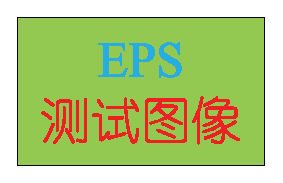
\includegraphics[width=0.3\textwidth]{chap2/testeps}}
  \hspace{1in}
  \subfigure[PDF Figure]{
    \label{fig:epspdf:b} %% label for second subfigure
    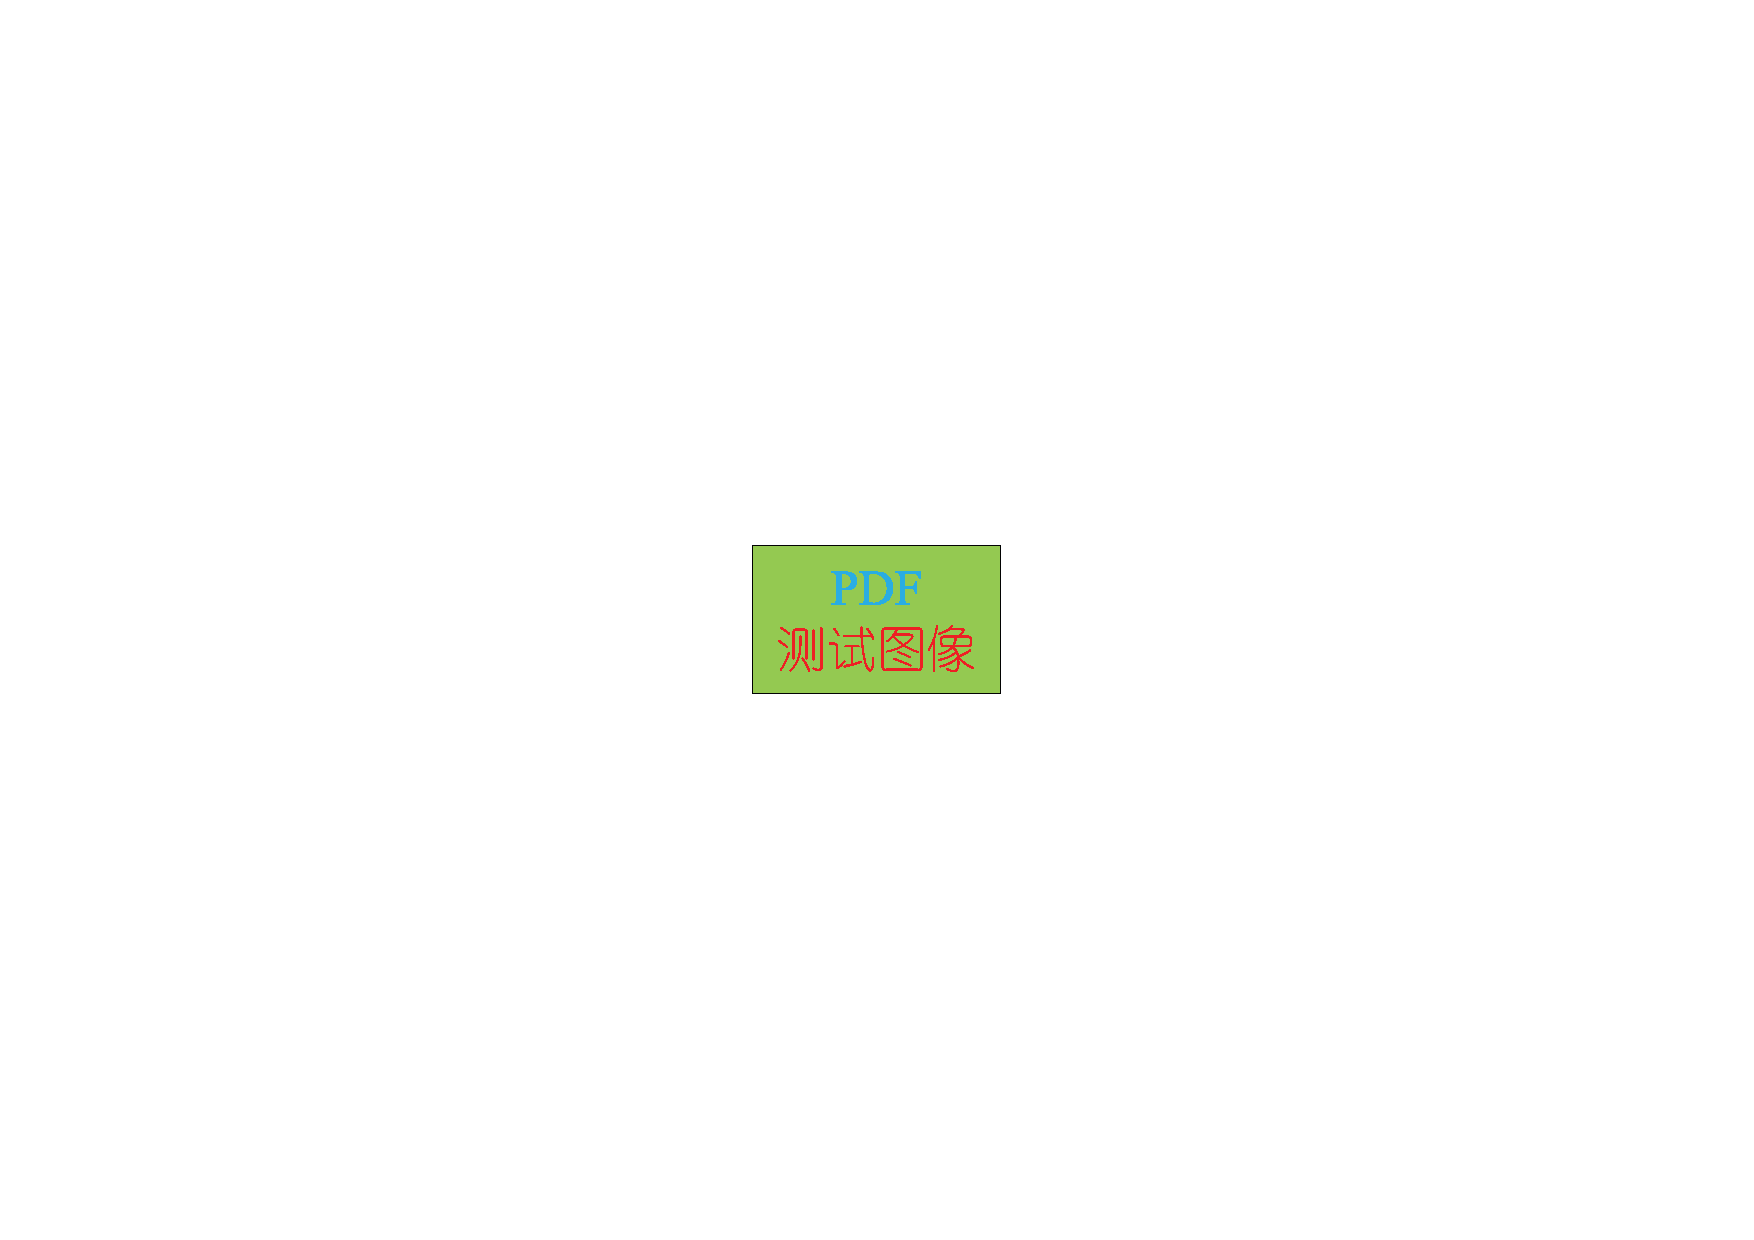
\includegraphics[angle=-90,origin=br,width=0.3\textwidth]{chap2/testpdf.pdf}}
  \bicaption[fig:pdfeps]{插入eps图像和pdf图像}{插入eps和pdf的例子}{Fig}{An EPS and PDF demo}
\end{figure}

更多关于~\LaTeX~插图的例子可以参考\href{http://www.cs.duke.edu/~junhu/Graphics3.pdf}{《~\LaTeX~插图指南》}。

\subsection{长标题的换行}
\label{sec:longcaption}

图\ref{fig:longcaptionbad}和图\ref{fig:longcaptiongood}都有比较长图标题,通过对比发现,图\ref{fig:longcaptiongood}的换行效果更好一些。
其中使用了minipage环境来限制整个浮动题的宽度。

\begin{figure}[!htp]
 \centering
 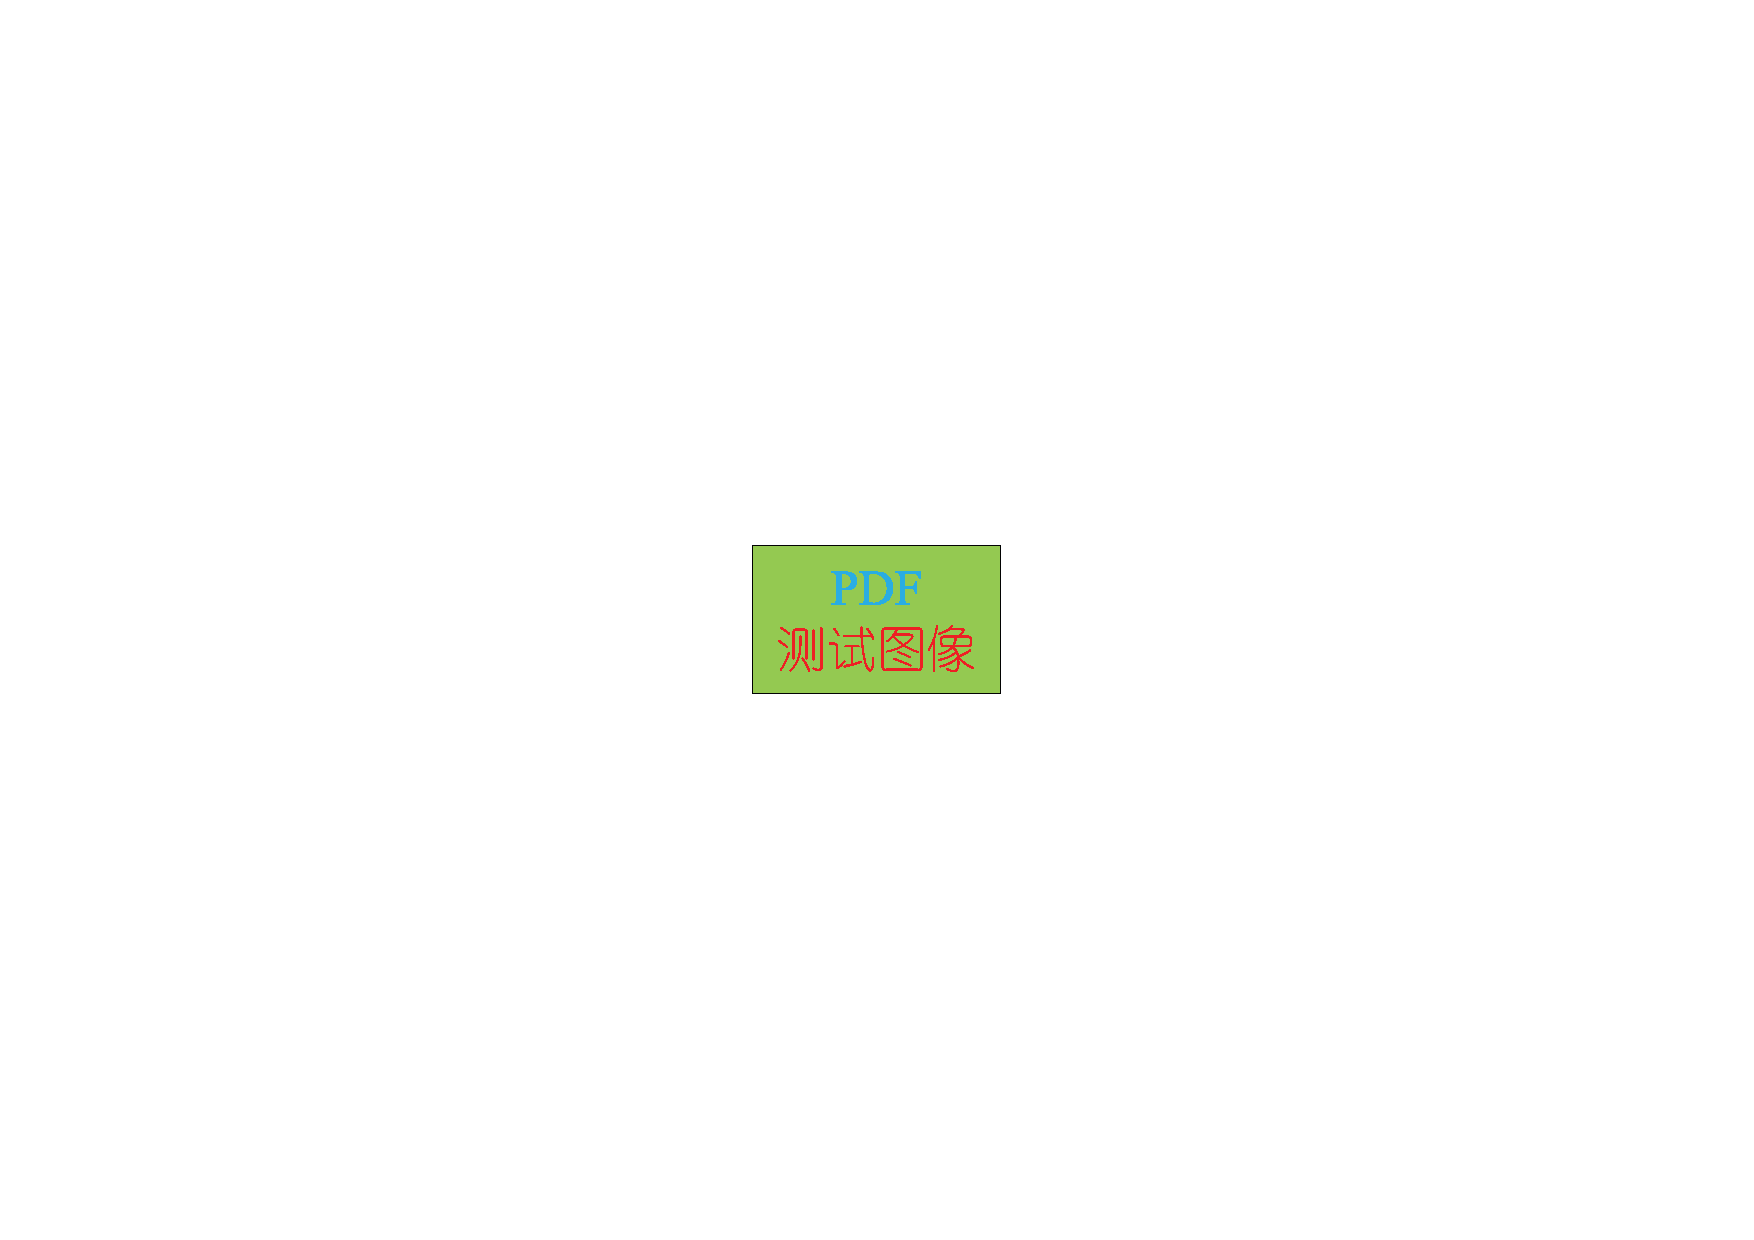
\includegraphics[angle=-90,origin=br,width=4cm]{chap2/testpdf.pdf}
 \bicaption[fig:longcaptionbad]{这里将出现在插图索引}{海交通大学是我国历史最悠久的高等学府之一,是教育部直属、教育部与上海市共建的全国重点大学.}{Fig}{Joomla! is one of the most powerful Open Source Content Management Systems on the planet.}
\end{figure}


  \begin{figure}[!hbp]
    \centering
    \begin{minipage}[b]{0.6\textwidth}
      \captionstyle{\centering}
      \centering
      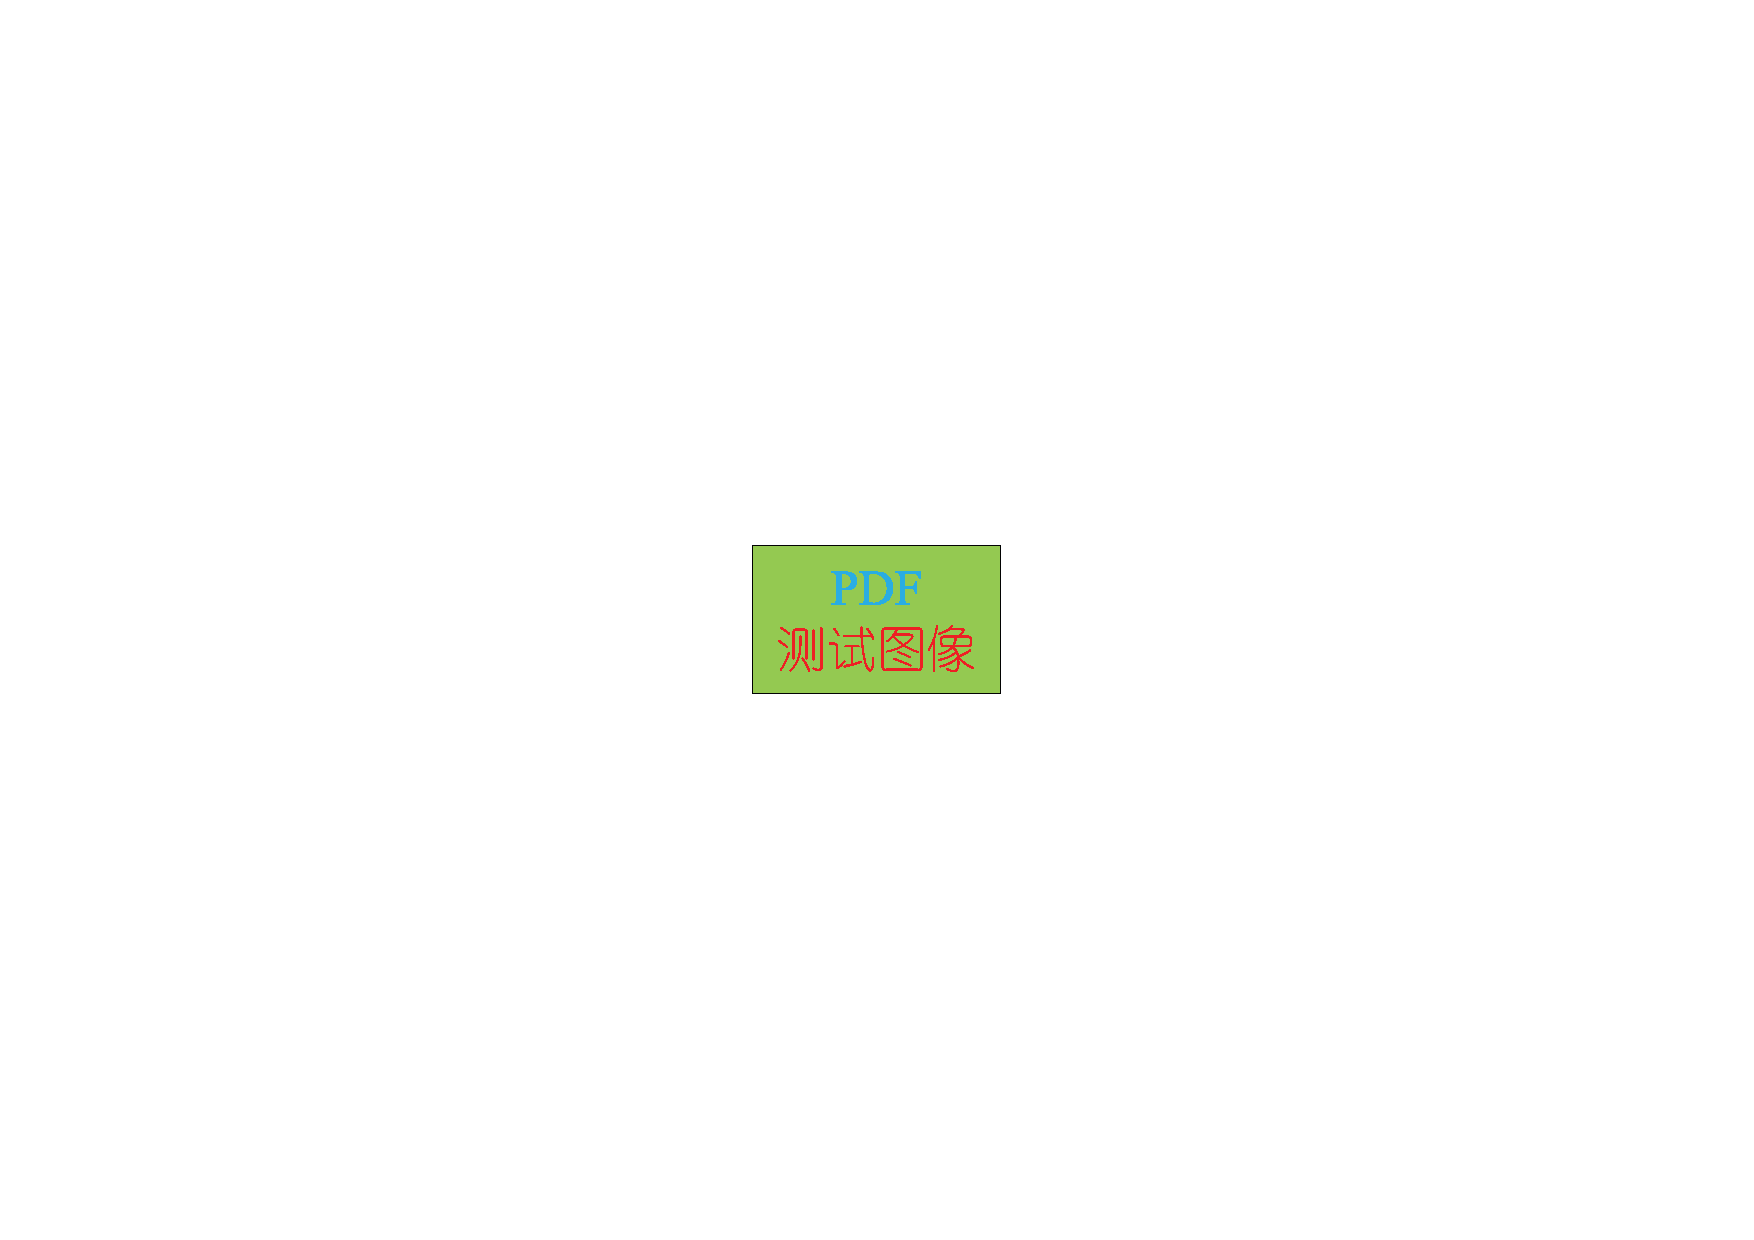
\includegraphics[angle=-90,origin=br,width=4cm]{chap2/testpdf.pdf}
      \bicaption[fig:longcaptiongood]{这里将出现在插图索引}{海交通大学是我国历史最悠久的高等学府之一,是教育部直属、教育部与上海市共建的全国重点大学.}{Fig}{Joomla! is one of the most powerful Open Source Content Management Systems on the planet.}
    \end{minipage}     
  \end{figure}

  
\section{表格的例子}
\label{sec:tab}

这一节给出的是一些表格的例子,如表\ref{tab:firstone}所示。

\begin{table}[!hpb]
  \centering
  \bicaption[tab:firstone]{指向一个表格的表目录索引}{一个颇为标准的三线表格\footnotemark[1]}{Table}{A Table}
  \begin{tabular}{@{}llr@{}} \toprule
    \multicolumn{2}{c}{Item} \\ \cmidrule(r){1-2}
    Animal & Description & Price (\$)\\ \midrule
    Gnat & per gram & 13.65 \\
    & each & 0.01 \\
    Gnu & stuffed & 92.50 \\
    Emu & stuffed & 33.33 \\
    Armadillo & frozen & 8.99 \\ \bottomrule
  \end{tabular}
\end{table}
\footnotetext[1]{这个例子来自\href{http://www.ctan.org/tex-archive/macros/latex/contrib/booktabs/booktabs.pdf}{《Publication quality tables in LATEX》}(booktabs宏包的文档)。这也是一个在表格中使用脚注的例子,请留意与threeparttable实现的效果有何不同。}

下面一个是一个更复杂的表格,用threeparttable实现带有脚注的表格,如表\ref{tab:footnote}。

\begin{table}[!htpb]
  \bicaption[tab:footnote]{出现在表目录的标题}{一个带有脚注的表格的例子}{Table}{A Table with footnotes}
  \centering
  \begin{threeparttable}[b]
     \begin{tabular}{ccd{4}cccc}
      \toprule
      \multirow{2}{6mm}{total}&\multicolumn{2}{c}{20\tnote{1}} & \multicolumn{2}{c}{40} &  \multicolumn{2}{c}{60}\\
      \cmidrule(lr){2-3}\cmidrule(lr){4-5}\cmidrule(lr){6-7}
      &www & k & www & k & www & k \\
      \midrule
      &$\underset{(2.12)}{4.22}$ & 120.0140\tnote{2} & 333.15 & 0.0411 & 444.99 & 0.1387 \\
      &168.6123 & 10.86 & 255.37 & 0.0353 & 376.14 & 0.1058 \\
      &6.761    & 0.007 & 235.37 & 0.0267 & 348.66 & 0.1010 \\
      \bottomrule
    \end{tabular}
    \begin{tablenotes}
    \item [1] the first note.% or \item [a]
    \item [2] the second note.% or \item [b]
    \end{tablenotes}
  \end{threeparttable}
\end{table}

\section{参考文献管理}

参考文献的管理是这个学位论文模板又一个好玩的地方。

\subsection{将参考文献的内容与表现分离}

这个论文模板使用BibTeX处理参考文献,这又是一个``内容''与``表现形式''分离的极好例子
\footnote{当然,你也可以手动编参考文献item,直接插入文档中。但是,有BibTeX帮助,我觉得没有人想用这种麻烦的方法,所以就在脚注中说明了。}。
参考文献的``内容''就是reference文件夹下的chap\textit{xx}.bib,参考文献的元数据(名称、作者、出处等)以一定的格式保存在这些纯文本文件中。
.bib文件也可以理解为参考文献的``数据库'',正文中所有引用的参考文件条目都会从这些文件中``析出''。
控制参考文献条目``表现形式''(格式)的是.bst文件。.bst文件定义了参考文献风格,使用不同的参考文献风格能将同一个参考文献条目输出成不同的格式。
当然,一个文档只能使用一个参考文献风格。
按照教务处的要求,本模板使用的是国标GBT7714风格的参考文献。

BibTeX的工作过程是这样的:
BibTeX读取.aux(第一次运行latex得到的)看看你引用了什么参考文献条目,
然后到.bib中找相关条目的信息,
最后根据.bst的格式要求将参考文献条目格式化输出,写到.bbl文件中。
在运行latex将.bbl插入文档之前,你可以用文本编辑器打开它,做一些小的修改。
你会发现,.bbl的格式和你自己手动写item很相似,它已经被赋予了一定的``表现形式''。

.bib数据库中的参考文献条目可以手动编写,也可以在google的学术搜索中找到。
各大数据库\footnote{应该说是国际知名数据库,譬如~SCOPUS, IEEE, OSA等,国内数据库在搜索、导出方面一直是差得一塌糊涂。}也支持将参考文献信息导出为.bib,
省时省力。
以Google学术搜索为例:进入\url{http://scholar.google.cn},在``学术搜索设置''中,将``文献管理软件''设为``显示导入BibTeX''的连接,保存退出。
然后学术搜索找到文献下会有``导出到BibTeX''连接,点击后Firefox会打开新的标签页,出现类似代码\ref{googlescholar}所示的内容
\footnote{展示这些.bib条目使用了listings宏包,因为listings宏包协调中文的能力很糟糕,所以读者在查看模板的这部分源代码时会看到一些非常麻烦的东西。并且,直接将源代码的这部分内容复制到.bib中可能还会出错。我的建议是:这部分内容留意PDF就足够了。}。
请注意,这个条目离``规范''还有一些距离。

  \begin{lstlisting}[caption={从Google Scholar找到的,但并不规范的.bib条目}, label=googlescholar, float, escapeinside="", numbers=none]
    @phdthesis{"白2008信用风险传染模型和信用衍生品的定价",
      title={{"信用风险传染模型和信用衍生品的定价"}},
      author={"白云芬"},
      year={2008},
      school={"上海交通大学"}
    } 
  \end{lstlisting}

  上面的.bib条目的``名字''\cndash{}``白2008信用风险传染模型和信用衍生品的定价'',包含~ASCII~以外的字符,BibTeX无法处理;
  条目还缺少了address域,这样编译出来的结果会出现``地址不详'';
  并且,条目还缺少language域,BibTeX需要language域来判断是否是中文参考文献。
  将上面的条目修正(改英文名、增加address和language域),复制到本地的.bib文件中就可以了。
  显然,这里描述的是参考文献的内容,而不是表现形式。

  \begin{lstlisting}[caption={一个符合规范的.bib条目}, label=itemok, float, escapeinside="", numbers=none]
    @phdthesis{bai2008,
      title={{"信用风险传染模型和信用衍生品的定价"}},
      author={"白云芬"},
      year={2008},
      language={zh},
      address={"上海"},
      school={"上海交通大学"}
    } 
  \end{lstlisting}

由于中英文参考文献处理起来有差异,所以需要在参考文献中标注是否是中文文献。
确切地说,BibTeX并不具有区分中英文参考文献的``智能'',这种智慧的来源是.bst文——它定义了处理参考文献的规则。
GBT7714-2005NLang.bst中规定:.bib中的条目,如果条目的``language''域非空,就被认为是中文文献,否则被认为是英文文献。
例如,刚才的文献,就会被认为是中文参考文献,采取一些针对中文的处理方式。

最后,这个条目被bibtex处理后,赋予了一定的``表现形式'',在.bbl文件中以下面的样子出现。
你还可以对它进行小的修改,这是一种很折磨人的终极修改方法。
再次运行latex之后,它将被插入到文档中。

\begin{lstlisting}[caption={.bbl中被格式化之后的条目}, escapeinside="", numbers=none]
\bibitem["白云芬(2008)"]{bai2008}
  \textsc{"白云芬"}.
  \newblock {"信用风险传染模型和信用衍生品的定价"}[D].
  \newblock "上海: 上海交通大学, 2008."
\end{lstlisting}

再罗嗦两句,
.bst文件书写起来非常繁杂\footnote{可以参考《Tame The BeaST》。},书写符合GBT7714标准的.bst文件更是一项浩大的工程。
因此,当大家为漂亮、标准的参考文献列表感到满意时,应该对GBT7714-2005NLang.bst的作者充满谢意。
作者在CTeX BBS发的帖子,请看
\href{http://bbs.ctex.org/viewthread.php?tid=33571&highlight=\%B2\%CE\%BF\%BC\%CE\%C4\%CF\%D7\%2BGB}{文后参考文献著录规则 GB/T 7714-2005}。
关于GB/T 7714-2005标准本身,请看\href{http://bbs.ctex.org/viewthread.php?tid=33571&highlight=GB\%2B\%B2\%CE\%BF\%BC\%CE\%C4\%CF\%D7}{这里}。

再多说两句,.bib是“参考文献的内容”,而控制参考文献表现(格式)的是.bst文件,本模板附带的是GBT7714-2005NLang.bst。

\subsection{在正文中引用参考文献}

参考文献可以分章节管理,只需要在主文件中的参考文献中都包含进去就可以,如\verb+\bibliography{chap1,chap2,...}+。

正文中引用参考文献时,用\verb+\upcite{key1,key2,key3...}+可以产生“上标引用的参考文献”,
如\upcite{Meta_CN,chen2007act,DPMG}。
使用\verb+\cite{key1,key2,key3...}+则可以产生水平引用的参考文献,例如\cite{JohnD,zhubajie,IEEE-1363}。
请看下面的例子,将会穿插使用水平的和上标的参考文献:关于书的\cite{Meta_CN,JohnD,IEEE-1363},关于期刊的\upcite{chen2007act,chen2007ewi},
会议论文\cite{DPMG,kocher99,cnproceed},
硕士学位论文\cite{zhubajie,metamori2004},博士学位论文\upcite{shaheshang,FistSystem01,bai2008},标准文件\cite{IEEE-1363},技术报告\upcite{NPB2},电子文献\cite{xiaoyu2001, CHRISTINE1998}。

最后总结一些注意事项:
\begin{itemize}
\item 参考文献只有在正文中被引用了,才会在最后的参考文献列表中出现;
\item 参考文献``数据库文件''.bib是纯文本文件,请使用~UTF-8~编码,不要使用~GBK~编码;
\item 参考文献条目中通过~language~域是否为空判断是否是中文文献;
\item 参考文献条目同样有“内容”和“表现形式”之分,这种可控性是BibTeX带来的。
\end{itemize}


\subsection{参考文献管理器}

参考文献数据库.bib虽然是纯文本的,可以用任意的文本编辑器查看,但总有人喜欢一个找一个``可视化''地查看每一条参考文献。
我想\href{http://jabref.sourceforge.net/}{JabRef}应该是个很不错的选择。
这是一个~Java~写的程序,需要~JRE~才能运行。
就我测试的情况上看,很幸运,JabRef可以顺利打开GBK编码的.bib文件。
但是,打开UTF--8编码的.bib源文件过程中总会崩溃,原因不得而知。
由于我们的~.bib~文件使用的是~UTF-8~编码,所以~JabRef~暂时不可用。

提到参考文献管理器,不得不提到另一个广被使用的软件——\href{http://www.endnote.com/}{EndNote}。
在图书馆的宣讲会上,EndNote被吹得神乎其神,但我发现他对.bib的管理很不友好。
EndNote可以导入.bib文件,却不能导出.bib,只能导出.bbl——被格式化的.bib。
原来,JabRef比较``单纯'',不具备格式化参考文献的能力;
而EndNote有那么一点设置参考文献输出格式的能力,然后就把这种能力滥用,这点搞得我很不爽。
看来,EndNote和Word配合得更好一些。


\section{用~listings~插入源代码}

原先~ctexbook~文档类和~listings~宏包配合使用时,代码在换页时会出现莫名其妙的错误,后来经高人指点,顺利解决了。
感兴趣的话,可以看看\href{http://bbs.ctex.org/viewthread.php?tid=53451}{这里}。
这里给使用~listings~宏包插入源代码的例子,这里是一段C代码。
另外,listings宏包真可谓博大精深,可以实现各种复杂、漂亮的效果,想要进一步学习的同学,可以参考
\href{http://mirror.ctan.org/macros/latex/contrib/listings/listings.pdf}{listings宏包手册}。

\begin{lstlisting}[language={C}, caption={一段C源代码}]
#include <stdio.h>
#include <unistd.h>
#include <sys/types.h>
#include <sys/wait.h>

int main() {
  pid_t pid;

  switch ((pid = fork())) {
  case -1:
    printf("fork failed\n");
    break;
  case 0:
    /* child calls exec */
    execl("/bin/ls", "ls", "-l", (char*)0);
    printf("execl failed\n");
    break;
  default:
    /* parent uses wait to suspend execution until child finishes */
    wait((int*)0);
    printf("is completed\n");
    break;
  }

  return 0;
}
\end{lstlisting}

再给一个插入MATLAB代码的例子,感谢~daisying~站友提供的代码。

\begin{lstlisting}[language={matlab}, caption={一段MATLAB源代码}]
function paper1
r=0.05;
n=100;
T=1;
X=1;
v0=0.8;
sigma=sqrt(0.08);
deltat=T/n;
for i=1:n
    t(i)=i*deltat;
    w(i)=random('norm',0,t(i),1);
end
for i=1:n
    alpha(i)=0.39;
end
for i=1:n
    temp=0;
    for k=1:i
        temp=temp+alpha(k);
    end
    B(i)=exp(r*t(i));
    BB(i)=B(i)*exp(temp*deltat);
    BBB(i)=exp(-r*(T-t(i)));
end
for i=1:n
    s0(i)=X*BBB(i);
    v(i)=v0*exp((r-0.5*sigma^2)*t(i)+sigma*w(i));
    for j=i+1:n
        D=X*BBB(j);
        d1=(log(v(i)/D)+(r+sigma^2/2)*(t(j)-t(i)))/(sigma*sqrt(t(j)-t(i)));
        d2=d1-(sigma*sqrt(t(j)-t(i)));
        ppp(i,j)=D*exp(-r*(t(j)-t(i)))*(1-cdf('normal',d2,0,1))-v(i)*(1-cdf('n
ormal',d1,0,1));
    end
end
for i=1:n
    s1(i)=0;
    for j=i+1:n
        s1(i)=s1(i)+BB(j)^(-1)*alpha(j)*deltat*(X*BBB(j)-B(j)/B(i)*ppp(i,j));
    end
    s2(i)=0;
    for j=1:n
        s2(i)=s2(i)+alpha(j);
    end
    s2(i)=X*exp(-r*T-s2(i)*deltat);
    s(i)=BB(i)*(s1(i)+s2(i));
end
plot(s)
hold on;
plot(s0);
\end{lstlisting}

%%==================================================
%% chapter03.tex for SJTU Master Thesis
%% based on CASthesis
%% modified by wei.jianwen@gmail.com
%% version: 0.3a
%% Encoding: UTF-8
%% last update: Dec 5th, 2010
%%==================================================

% \bibliographystyle{sjtu2} %[此处用于每章都生产参考文献]

\chapter{已知问题}
\label{chap:needsomehelp}

自谦一下,由于时间非常仓促,这个模板肯定存在不少问题,所以我需要大家帮助一起解决这些问题。下面是我自认为模板需要改进的地方。

\subsubsection*{这模板有点丑}
我自己也觉得这个模板的版面设计有点不和谐,离一个“工整严谨”的科技论文模板还有一段距离,但是不知道是什么地方出了问题。我工科男一个,宅男一枚,欢迎来信指正版面设计事宜。

\subsubsection*{你的~Makefile~不管用啊}
是的,因为BibTeX编译出现错误,make~时总是退出,我也不知道咋办。希望大家帮帮忙。



%%==================================================
%% chapter04.tex for SJTU Master Thesis
%% based on CASthesis
%% modified by wei.jianwen@gmail.com
%% version: 0.3a
%% Encoding: UTF-8
%% last update: Dec 5th, 2010
%%==================================================

% \bibliographystyle{sjtu2} %[此处用于每章都生产参考文献]

\chapter{常被问到和不常被问到的问题}
\label{chap:faq}

\subsubsection*{我是否能够自由使用这份模板}
是的,你可以爱咋用就咋用。拿去卖钱的话麻烦先通知我一声,我得先把里面的~Bugs~剔除干净。

\subsubsection*{我的论文是~Word~排版的,学校图书馆是不是只收~\LaTeX~排版的论文}
显然不是,Word~版肯定收。

\subsubsection*{我的论文是~\LaTeX~排版的,学校图书馆是不是只收~Word~排版的论文}
显然不是,PDF~版的电子论文也是可以上交的。是否要交~Word~版就看你导师的喜好了。

\subsubsection*{为什么左右页边距不一样}
模板默认是双面打印,迎面页和背面页的页边距是要交换的,多出来的那一部分是留作装订的。

\subsubsection*{为什么在参考文献中会有``//''符号}
那是国标~GBT7714~参考文献风格规定的,如果下次有人怀疑``//''不合规范,你可以鄙视TA了。

\subsubsection*{为什么参考文献中会有[s.n.],[S.l], [EB/OL]等符号}
那也是国标~GBT7714~参考文献风格定义的。[s.n.]表示出版者不祥,[S.l]表示出版地不祥,[EB/OL]表示引用的参考文献类型为在线电子文档。

\subsubsection*{如何获得帮助和反馈意见}
你可以通过查看文档、到TeX\_LaTeX版发帖来获得帮助。如果你觉得你的意见足够高明,可以直接给我\href{mail:wei.jianwen@gmail.com}{发邮件}。

\subsubsection*{你做这个是有偿劳动吗}
我做这个模板是无偿劳动。

\subsubsection*{如何向你表示感谢}
口头感谢、站内感谢、\href{wei.jianwen@gmail.com}{MSN感谢}、送锦旗、请吃饭、写入你论文致谢都可以,但最好你能帮我解决第\ref{chap:needsomehelp}章中的问题。谢谢大家。


\chapter*{ȫ���ܽ�\markboth{ȫ���ܽ�}{}}
\addcontentsline{toc}{chapter}{ȫ���ܽ�}

������ȫ���ܽ����ݡ�

 %% 全文总结


%%%%%%%%%%%%%%%%%%%%%%%%%%%%%% 
%% 附录(章节编号重新计算,使用字母进行编号)
%%%%%%%%%%%%%%%%%%%%%%%%%%%%%% 
\appendix

% 附录中编号形式是"A-1"的样子
\renewcommand\theequation{\Alph{chapter}--\arabic{equation}}
\renewcommand\thefigure{\Alph{chapter}--\arabic{figure}}
\renewcommand\thetable{\Alph{chapter}--\arabic{table}}

\chapter{ģ����¼�¼}
\label{chap:updatelog}

\begin{itemize}
\item[2009��11��20�գ�] v0.2a�������ο����׷����ù���GBT7714�������˲����������ӣ�������ģ��ʹ��˵����
\item[2009��10��26�գ�] �ο����׷������廪��ѧѧλ����ģ���е�thubib.bst���ڲο�����ʾ���������˶������͵IJο��������ӣ�ɾ����ԭ��ģ���й����ظ��IJ��֡�v0.1b������׼����һ�汾��
\item[2009��10��16�գ�] ��������һЩ���޲����Ĺ�����v0.1a������׼����һ�汾v0.1b��
\item[����֮ǰ��] ����ϵ������ͬѧ�����˻���~CASthesis~�IJ�ʿѧλ����ģ��
\end{itemize}
 % 更新记录
%% app2.tex for SJTU Master Thesis
%% based on CASthesis
%% modified by wei.jianwen@gmail.com
%% version: 0.3a
%% Encoding: UTF-8
%% last update: Dec 5th, 2010
%%==================================================

\chapter{Maxwell Equations}

选择二维情况,有如下的偏振矢量
\begin{subequations}
  \begin{eqnarray}
    {\bf E}&=&E_z(r,\theta)\hat{\bf z} \\
    {\bf H}&=&H_r(r,\theta))\hat{ \bf r}+H_\theta(r,\theta)\hat{\bm
      \theta}
  \end{eqnarray}
\end{subequations}
对上式求旋度
\begin{subequations}
  \begin{eqnarray}
    \nabla\times{\bf E}&=&\frac{1}{r}\frac{\partial E_z}{\partial\theta}{\hat{\bf r}}-\frac{\partial E_z}{\partial r}{\hat{\bm\theta}}\\
    \nabla\times{\bf H}&=&\left[\frac{1}{r}\frac{\partial}{\partial
        r}(rH_\theta)-\frac{1}{r}\frac{\partial
        H_r}{\partial\theta}\right]{\hat{\bf z}}
  \end{eqnarray}
\end{subequations}
因为在柱坐标系下,$\overline{\overline\mu}$是对角的,所以Maxwell方程组中电场$\bf
E$的旋度
\begin{subequations}
  \begin{eqnarray}
    &&\nabla\times{\bf E}=\mathbf{i}\omega{\bf B} \\
    &&\frac{1}{r}\frac{\partial E_z}{\partial\theta}{\hat{\bf
        r}}-\frac{\partial E_z}{\partial
      r}{\hat{\bm\theta}}=\mathbf{i}\omega\mu_rH_r{\hat{\bf r}}+\mathbf{i}\omega\mu_\theta
    H_\theta{\hat{\bm\theta}}
  \end{eqnarray}
\end{subequations}
所以$\bf H$的各个分量可以写为:
\begin{subequations}
  \begin{eqnarray}
    H_r=\frac{1}{\mathbf{i}\omega\mu_r}\frac{1}{r}\frac{\partial
      E_z}{\partial\theta } \\
    H_\theta=-\frac{1}{\mathbf{i}\omega\mu_\theta}\frac{\partial E_z}{\partial r}
  \end{eqnarray}
\end{subequations}
同样地,在柱坐标系下,$\overline{\overline\epsilon}$是对角的,所以Maxwell方程组中磁场$\bf
H$的旋度
\begin{subequations}
  \begin{eqnarray}
    &&\nabla\times{\bf H}=-\mathbf{i}\omega{\bf D}\\
    &&\left[\frac{1}{r}\frac{\partial}{\partial
        r}(rH_\theta)-\frac{1}{r}\frac{\partial
        H_r}{\partial\theta}\right]{\hat{\bf
        z}}=-\mathbf{i}\omega{\overline{\overline\epsilon}}{\bf
      E}=-\mathbf{i}\omega\epsilon_zE_z{\hat{\bf z}} \\
    &&\frac{1}{r}\frac{\partial}{\partial
      r}(rH_\theta)-\frac{1}{r}\frac{\partial
      H_r}{\partial\theta}=-\mathbf{i}\omega\epsilon_zE_z
  \end{eqnarray}
\end{subequations}
由此我们可以得到关于$E_z$的波函数方程:
\begin{eqnarray}
  \frac{1}{\mu_\theta\epsilon_z}\frac{1}{r}\frac{\partial}{\partial r}
  \left(r\frac{\partial E_z}{\partial r}\right)+
  \frac{1}{\mu_r\epsilon_z}\frac{1}{r^2}\frac{\partial^2E_z}{\partial\theta^2}
  +\omega^2 E_z=0
\end{eqnarray}
 % 麦克斯韦方程
% \include{body/app3}


%%%%%%%%%%%%%%%%%%%%%%%%%%%%%% 
%% 文后(无章节编号)
%%%%%%%%%%%%%%%%%%%%%%%%%%%%%% 
\backmatter

% 参考文献
% 使用 BibTeX
% 包含参考文献文件.bib
\bibliography{reference/chap1,reference/chap2}

%% 个人简历(硕士学位论文没有个人简历要求)
% %%==================================================
%% resume.tex for SJTU Master Thesis
%% based on CASthesis
%% modified by wei.jianwen@gmail.com
%% version: 0.3a
%% Encoding: UTF-8
%% last update: Dec 5th, 2010
%%==================================================

\begin{resume}

\begin{resumesection}{基本情况}
xxx,男,上海人,1985 年~12 月出生,未婚,
上海交通大学物理系在读博士研究生。
\end{resumesection}

\begin{resumelist}{教育状况}
XXXX 年~9 月至~XXXX 年~7 月,上海交通大学, 本科,专业:XXXX

XXXX 年~9 月至~XXXX 年~7 月,上海交通大学, 硕士研究生,专业:XXXX

XXXX 年~9 月至~XXXX 年~7 月,上海交通大学,
博士研究生(提前攻读博士),专业:XXXX
\end{resumelist}

\begin{resumelist}{工作经历}
无。
\end{resumelist}

\begin{resumelist}{研究兴趣}
XXXXXXX。
\end{resumelist}

\begin{resumelist}{联系方式}
通讯地址:上海市闵行区东川路800号,上海交通大学物理系

邮编:200240

E-mail: abcde@sjtu.edu.cn
\end{resumelist}

\end{resume}


% 致谢
\begin{thanks}

ֵ���������֮�ʣ����ڴ�������������ҹ��ĺͰ�������ʦ��ͬѧ�����Ѻͼ��˱�ʾ���ĵĸ�л��

ֵ���������֮�ʣ����ڴ�������������ҹ��ĺͰ�������ʦ��ͬѧ�����Ѻͼ��˱�ʾ���ĵĸ�л��

ֵ���������֮�ʣ����ڴ�������������ҹ��ĺͰ�������ʦ��ͬѧ�����Ѻͼ��˱�ʾ���ĵĸ�л��

��л�Ϻ����󣬸�лCCTV����л�����������ᡭ��

\vskip 18pt

���ѱ����׸��������ҵ�ĸ�ף�

\vfill

\noindent\small{$^{\dag}$ ��������~\LaTeXe~�Ű棬����ģ���޸���~$\mathbb{C}$\TeX~��վ��~\texttt{CASthesis}~ģ��}

\end{thanks}


% 发表文章目录
%%==================================================
%% pub.tex for SJTU Master Thesis
%% based on CASthesis
%% modified by wei.jianwen@gmail.com
%% version: 0.3a
%% Encoding: UTF-8
%% last update: Dec 5th, 2010
%%==================================================

\begin{publications}{99}

    \item\textsc{Chen H, Chan C~T}. {Acoustic cloaking in three dimensions using acoustic metamaterials}[J].
      Applied Physics Letters, 2007, 91:183518.

    \item\textsc{Chen H, Wu B~I, Zhang B}, et al. {Electromagnetic Wave Interactions with a Metamaterial Cloak}[J].
      Physical Review Letters, 2007, 99(6):63903.
    
\end{publications}


% 参与项目列表
%%==================================================
%% projects.tex for SJTU Master Thesis
%% based on CASthesis
%% modified by wei.jianwen@gmail.com
%% version: 0.3a
%% Encoding: UTF-8
%% last update: Dec 5th, 2010
%%==================================================

\begin{projects}{99}

    \item 973项目“XXX”
    \item 自然基金项目“XXX”
    \item 国防项目“XXX”
    
\end{projects}


\end{document}
